\documentclass[12pt]{article}
\usepackage{lecture}
\usepackage{html}
\usepackage{url}
\usepackage{graphics}
\usepackage{epstopdf}

\newcommand{\copyrightYears}{2001-2015}

\title{The Coalescent}

\begin{document}

\maketitle

\thispagestyle{first}

\section*{Introduction}

I've mentioned many times by now that population geneticists often
look at the world backwards. Sometimes when they do, the result is
very useful. Consider genetic drift, for example. So far we've been
trying to predict what will happen in a population given a particular
effective population size. But when we collect data we are often more
interested in understanding the processes that produced the pattern we
find than in predicting what will happen in the future. So let's take
a backward look at drift and see what we find.


\section*{Reconstructing the genealogy of a sample of
  alleles}\index{allele genealogy}\index{coalescent}

Specifically, let's keep track of the genealogy of alleles. In a
finite population, two randomly chosen alleles will be identical by
descent with respect to the immediately preceding generation with
probability $1/2N_e$. That means that there's a chance that two
alleles in generation $t$ are copies of the same allele in generation
$t-1$. If the population size is constant, meaning that the number of
alleles in the population is remaining constant, then there's also a
chance that some alleles present in generation $t-1$ will not have
descendants in generation $t$. Looking backward, then, the number of
alleles in generation $t-1$ that have descendants in generation $t$ is
always less than or equal to the number of alleles in generation
$t$. That means if we trace the ancestry of alleles in a sample back
far enough, all of them will be descended from a single common
ancestor. Figure~\ref{fig:coalescent} provides a simple schematic
illustrating how this might happen.

\begin{figure}
\begin{center}
\resizebox{!}{5cm}{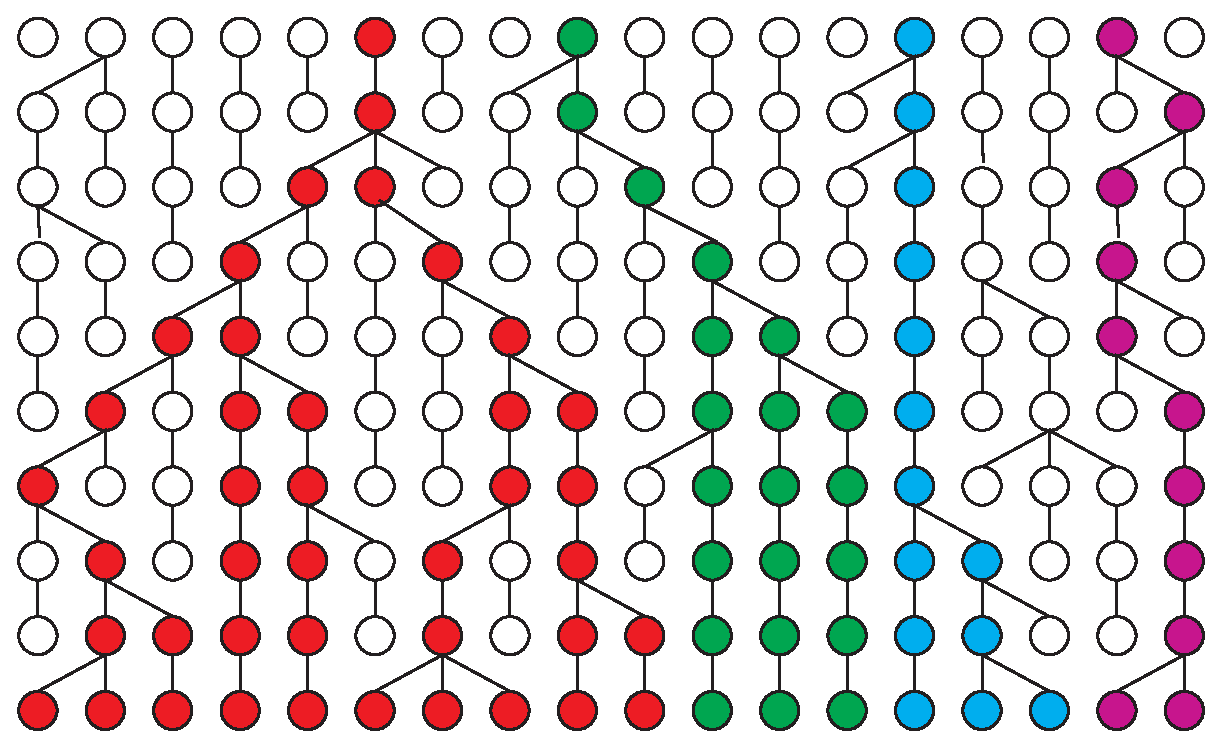
\includegraphics{coalescent-figure.eps}}
\end{center}
\caption{A schematic depiction of one possible realization of the
  coalescent process in a population with 18 haploid gametes. There
  are four coalescent events in the generation immediately preceding
  the last one illustrated, one involving three alleles.}\label{fig:coalescent}
\end{figure}

Now take a look at Figure~\ref{fig:coalescent}. Time runs from the top
of the figure to the bottom, i.e., the current generation is
represented by the circles in the botton row of the figure. Each
circle represents an allele. The eighteen alleles in our current
sample are descended from only four alleles that were present in the
populations ten generations ago. The other fourteen alleles present in
the population ten generations ago left no descendants. How far back
in time we'd have to go before all alleles are descended from a single
common ancestor depends on the effective size of the population, and
how frequently two (or more) alleles are descended from the same
allele in the preceding generation depends on the effective size of
the population, too. But in any finite population the pattern will
look something like the one I've illustrated here.

\section*{Mathematics of the coalescent: two
  alleles}\index{coalescent!two alleles}

J. F. C. Kingman developed a convenient and powerful way to describe
how the time to common ancestry is related to effective population
size~\cite{Kingman-1982-genealogy,Kingman-1982-coalescent}. The
process he describes is referred to as the {\it coalescent}, because
it is based on describing the probability of {\it coalescent
  events},\index{coalescent events} i.e., those points in the
genealogy of a sample of alleles where two alleles are descended from
the same allele in the immediately preceding generation.\footnote{An
  important assumption of the coalescent is that populations are large
  enough that we can ignore the possibility that there is more than
  one coalescent event in a single generation. We also only allow
  coalescence between a pair of alleles, not three or more. In both
  ways the mathematical model of the process differs from the diagram
  in Figure~\ref{fig:coalescent}.}  Let's consider a simple case, one
that we've already seen, first, i.e., two alleles drawn at random from
a single populations.

The probability that two alleles drawn at random from a population are
copies of the same allele in the preceding generation is also the
probability that two alleles drawn at random from that population are
identical by descent with respect to the immediately preceding
generation. We know what that probability is,\footnote{Though you may
not remember it.} namely
\[
\frac{1}{2N_e^{(f)}} \quad .
\]
I'll just use $N_e$ from here on out, but keep in mind that the
appropriate population size for use with the coalescent is the
inbreeding effective size. Of course, this means that the probability
that two alleles drawn at random from a population are {\it not\/}
copies of the same allele in the preceding generation is
\[
1 - \frac{1}{2N_e} \quad .
\]
We'd like to calculate the probability that a coalescent event
happened at a particular time $t$, in order to figure out how far back
in the ancestry of these two alleles we have to go before they have a
common ancestor. How do we do that?

Well, in order for a coalescent event to occur at time $t$, the two
alleles must have {\it not\/} have coalesced in the generations
preceding that.\footnote{Remember that we're counting generations
  backward in time, so when I say that a coalescent event occurred at
  time $t$ I mean that it occurred $t$ generations ago.} The
probability that they did not coalesce in the first $t-1$ generations
is simply
\[
\left(1 - \frac{1}{2N_e}\right)^{t-1} \quad .
\]
Then after having remained distinct for $t-1$ generations, they have
to coalesce in generation $t$, which they do with probability
$1/2N_e$. So the probability that two alleles chosen at random
coalesced $t$ generations ago is
\begin{equation}
P(T=t) = \left(1 -
\frac{1}{2N_e}\right)^{t-1}\left(\frac{1}{2N_e}\right) \quad .
\label{eq:two-allele}
\end{equation}
It's not too hard to show, once we know the probability distribution
in equation (\ref{eq:two-allele}), that the average time to
coalescence for two randomly chosen alleles is $2N_e$.\footnote{If
  you've had a little bit of probability theory, you'll notice that
  equation~\ref{eq:two-allele} shows that the coalescence time is a
  geometric random variable.}

\section*{Mathematics of the coalescent: multiple
  alleles}\index{coalescent!multiple alleles}

It's quite easy to extend this approach to multiple
alleles.\footnote{Okay, okay. What I should really have said is ``It's
not {\it too\/} hard to extend this approach to multiple alleles.''}
We're interested in seeing how far back in time we have to go before
all alleles are descended from a single common ancestor. We'll assume
that we have $m$ alleles in our sample. The first thing we have to
calculate is the probability that any two of the alleles in our sample
are identical by descent from the immediately preceding generation. To
make the calculation easier, we assume that the effective size of the
population is large enough that the probability of two coalescent
events in a single generation is vanishingly small. We already know
that the probability of a coalescence in the immediately preceding
generation for two randomly chosen alleles is $1/2N_e$. But there are
$m(m-1)/2$ different pairs of alleles in our sample. So the
probability that one pair of these alleles is involved in a coalescent
event in the immediately preceding generation is
\[
\left(\frac{1}{2N_e}\right)\left(\frac{m(m-1)}{2}\right) \quad .
\]
From this it follows\footnote{Using logic just like what we used in
the two allele case.} that the probability that the first coalescent
event involving this sample of alleles occurred $t$ generations ago is
\begin{equation}
P(T=t) = 
\left(1-\left(\frac{1}{2N_e}\right)\left(\frac{m(m-1)}{2}\right)\right)^{t-1}
\left(\frac{1}{2N_e}\right)\left(\frac{m(m-1)}{2}\right)
\quad .
\label{eq:multi-allele}
\end{equation}
So the mean time back to the first coalescent event is
\[
\frac{2N_e}{m(m-1)/2} = \frac{4N_e}{m(m-1)} \hbox{ generations} \quad .
\]

But this is, of course, only the first coalescent event. We were
interested in how long we have to wait until {\it all\/} alleles are
descended from a single common ancestor. Now this is where Kingman's
sneaky trick comes in. After the first coalescent event, we have $m-1$
alleles in our sample, instead of $m$. So the whole process starts
over again with $m-1$ alleles instead of $m$. Since the time to the
first coalescence depends only on the number of alleles in the sample
and not on how long the first coalescence event took, we can calculate
the average time until all coalescences have happened
as\index{coalescent!time to coalescence}
\begin{eqnarray*}
\bar t &=& \sum_{k=2}^m \bar t_k \\
       &=& \sum_{k=2}^m \frac{4N_e}{k(k-1)} \\
       && \mbox{TAMO} \\
       &=& 4N_e\left(1 - \frac{1}{m}\right) \\
       &\approx& 4N_e
\end{eqnarray*}


\subsection*{An example: Mitochondrial
  Eve}\index{coalescent!mitochondrial Eve}

Cann et al.~\cite{Cann-etal-1987} sampled mitochondrial DNA from 147
humans of diverse racial and geographic origins. Based on the amount
of sequence divergence they found among genomes in their sample and
independent estimates of the rate of sequence evolution, they inferred
that the mitochondria in their sample had their most recent common
ancestor about 200,000 years ago. Because all of the most ancient
lineages in their sample were from individuals of African ancestry,
they also suggested that mitochondrial Eve lived in Africa. They used
these arguments as evidence for the ``Out of Africa'' hypothesis for
modern human origins, i.e., the hypothesis that anatomically modern
humans arose in Africa about 200,000 years ago and displaced other
members of the genus {\it Homo\/} in Europe and Asia as they
spread. What does the coalescent tell us about their conclusion?

Well, we expect all mitochondrial genomes in the sample to have had a
common ancestor about $2N_e$ generations ago. Why $2N_e$ rather than
$4N_e$? Because mitochondrial genomes are haploid. Furthermore, since
we all got our mitochondria from our mothers, $N_e$ in this case
refers to the effective number of {\it females}.

Given that a human generation is about 20 years, a coalescence time of
200,000 years implies that the mitochondrial genomes in the Cann et
al. sample have their most recent common ancestor about 10,000
generations ago. If the effective number of females in the human
populations is 5000, that's exactly what we'd expect. While 5000 may
sound awfully small, given that there are more than 3 billion women on
the planet now, remember that until the recent historical past (no
more than 500 generations ago) the human population was small and
humans lived in small hunter-gatherer groups, so an effective number
of females of 5000 and a total effective size of 10,000 may not be
unreasonable. If that's true, then the geographical location of
mitochondrial Eve need not tell us anything about the origin of modern
human populations, because there had to be a coalescence
somewhere. There's no guarantee, from this evidence alone, that the
Y-chromosome Adam would have lived in Africa, too. Having said that,
my limited reading of the literature suggests that other dara are
consistent with the ``Out of Africa'' scenario. Y-chromosome
polymorphisms, for example, are also consistent with the ``Out of
Africa'' hypothesis~\cite{Underhill-etal-2000}. Interestingly, dating
of those polymorphisms suggetsts that Y-chromosome Adam left Africa
35,000 -- 89,000 years ago.

\section*{The coalescent and $F$-statistics}\index{F-statistics@$F$-statistics!coalescent}\index{coalescent!F-statistics@$F$-statistics}

Suppose we have a sample of alleles from a structured population. For
alleles chosen randomly within populations let the average time to
coalescence be $\bar t_0$. For alleles chosen randomly from different
populations let the average time to coalescence be $\bar t_1$. If
there are $k$ populations in our sample, the average time to
coalescence for two alleles drawn at random without respect to
population is\footnote{If you don't see why, don't worry about it. You
can ask if you really care. We only care about $\bar t$ for what
follows anyway.}
\[
\bar t = \frac{k(k-1)\bar t_1 + k\bar t_0}
              {k} \quad .
\]
Slatkin~\cite{Slatkin-1991} pointed out that $F_{st}$ bears a simple
relationship to average coalescence times within and among
populations. Given these definitions of $\bar t$ and $\bar t_0$,
\[
F_{st} = \frac{\bar t - \bar t_0}{\bar t} \quad .
\]
So another way to think about $F_{st}$ is as a measure of the
proportional increase in coalescence time that is due to populations
being separate from one another. One way to think about that
relationship is this: the longer it has been, on average, since
alleles in different populations diverged from a common ancestor, the
greater the chances that they have become different. An implication of
this relationship is that $F$-statistics, by themselves, can tell us
something about how recently populations have been connected, relative
to the within-population coalescence time, but they can't distinguish
between recent common ancestry that is due to lots of migration among
populations and recent common ancestry that is due to a recent split
between populations.

A given pattern of among-population relationships might reflect a
migration-drift equilibrium, a sequence of population splits followed
by genetic isolation, or any combination of the two. If we are willing
to assume that populations in our sample have been exchanging genes
long enough to reach stationarity in the drift-migration process, then
$F_{st}$ may tell us something about migration. If we are willing to
assume that there's been no gene exchange among our populations, we
can infer something about how recently they've diverged from one
another. But unless we're willing to make one of those assumptions, we
can't really say anything.

\bibliography{popgen}
\bibliographystyle{plain}

\ccLicense

\end{document}
